\section{What industrial organization studies}\label{sec:01-what-is-io}

\emph{Industrial organization} (IO) is the field of economics that studies how industries are organized and
how firms and consumers behave within them. In the words of \citet[p.~146]{EinavLevin2010}, the field ``is
concerned with the structure of industries in the economy and the behavior of firms and individuals in these
industries.'' Its distinctive focus is on markets that depart from \emph{perfect competition}, the benchmark
in which many small firms take the price as given and price equals marginal cost. Such departures arise from
scale economies, transaction costs, strategic behavior and other frictions \citep[p.~146]{EinavLevin2010}.

The traditional questions of IO concern competition policy, regulation, and the determinants and consequences
of market power. Competition policy asks, for example, whether a merger will raise prices or whether a group of
sellers is fixing prices. Regulation asks how to set prices and entry rules in industries with large scale
economies, such as electricity transmission or local telephone service. The study of \emph{market power}, the
ability of a firm to keep its price above the competitive level, asks where such power comes from and what it
costs consumers. Each of these questions requires a model of how firms interact. A firm's best price depends on
the prices of its rivals, and a merger changes the incentives of the merging firms and of every firm that
competes with them.

The field therefore looks mostly at what happens between firms. What happens inside a firm, such as how it
organizes production or designs incentives for its employees, belongs largely to other fields. Productivity is
the main exception. Many IO economists measure productivity and study how competition and the selection of
efficient firms shape it. This book does not cover productivity.

Empirical IO relies on economic theory more than most other fields of applied microeconomics. We see two
reasons. The first is that theory has a great deal to say about firms and markets. Firms that set prices every
day plausibly come close to maximizing profit, and profit maximization in equilibrium imposes sharp
restrictions on data. \citet[pp.~158--159]{EinavLevin2010} draw the contrast with research on education.
Standard theory says little about how third graders learn. For firms and markets, they argue, theory ``has a
lot to say and, when appropriately used, generally serves to clarify rather than to complicate one's
understanding of a market.'' The second reason is historical. IO had a head start on the econometric modeling
of strategic behavior. By the late 1980s a body of work already estimated demand, cost and the form of
competition jointly within single industries, and \citet{Bresnahan1989} could survey it. A further
consideration reinforces both reasons. Many IO questions concern events that have not yet happened, such as a
proposed merger, and only a model of the industry can predict their effects.

These tools now travel beyond the traditional boundaries of the field. IO-trained economists study insurers
and hospitals in health care, schools and colleges in education, and banks and lenders in finance. Questions
about competition have become central in each of these sectors. The same methods serve markets with \emph{adverse
selection}, such as insurance, where the customers most eager to buy are the most costly to serve. They also
serve platforms that bring two groups of users together. \citet[p.~149]{EinavLevin2010}
report that the demand models developed in \cref{ch:aids,ch:discrete,ch:logit,ch:blp} have spread into trade,
education, housing, health and environmental economics. Economists sometimes call this expansion ``IO+.'' The
editors of the latest Handbook of Industrial Organization describe the same trend \citep[Preface, p.~xv]{HoHortacsuLizzeri2021}.
In their account, the ``econometric revolution'' that began with the New Empirical Industrial Organization of
\cref{sec:01-neio} has kept maturing. Its toolbox now reaches credit and insurance markets, financial markets, health
care, the energy sector and the environment.

Empirical IO also has a large footprint in policy and business. Its methods are used in merger reviews and
antitrust litigation, in regulatory decisions, in price setting by retailers, and in the design of auctions and
marketplaces \citep[p.~145]{EinavLevin2010}. Antitrust agencies and courts use demand estimates to define
markets, to simulate the price effects of mergers, and to compute damages from excessive prices
\citep[p.~149]{EinavLevin2010}. Around 1980, antitrust arguments often rested on simple concentration measures.
Today the agencies routinely commission econometric studies of the industry under review
\citep[p.~152]{EinavLevin2010}. Welfare measures derived from estimated demand have shaped the debate over how
the Consumer Price Index should account for new goods \citep[p.~149]{EinavLevin2010}. Empirical studies of
bidding have informed the regulation of wholesale electricity markets \citep[p.~154]{EinavLevin2010}. We treat
merger analysis in \cref{ch:mergers}, new goods in \cref{ch:newgoods}, and auctions in
\cref{ch:auction-theory,ch:auction-empirics}.

Almost every question in this book comes back to three objects, which we call the \emph{primitives} of a
market. The first is \emph{demand}, which describes how many units consumers buy at each price and how they
substitute between products. The second is \emph{cost}, in particular the \emph{marginal cost} of producing one
more unit. The third is \emph{conduct}, the way firms compete. Firms may set prices or quantities, act
independently or coordinate, and look ahead to rivals' reactions or ignore them. Price equals marginal cost
plus a markup, and the markup depends on demand and on conduct:
\begin{equation}\label{eq:01-price-decomposition}
  \text{price} = \text{marginal cost} + \text{markup}(\text{demand}, \text{conduct}).
\end{equation}
\Cref{sec:01-lerner,sec:01-cournot-hhi} make this decomposition precise.

In most data sets none of the three primitives is observed directly. We observe prices and quantities, which
are equilibrium outcomes. Each observed pair lies on the demand curve and on the firms' pricing rule at the
same time, so a scatter of prices and quantities traces out neither of them. \Cref{ch:aids,ch:logit} treat
this simultaneity problem. Accounting data record average and historical costs, with overhead allocated by
convention. \citet[p.~151]{EinavLevin2010}, following \citet{Bresnahan1989}, stress that accounting practices
are not designed to report the economic notion of marginal cost. Conduct is recorded nowhere, and firms that
coordinate have every reason to hide it. The history of empirical IO, told in the rest of this chapter, is a
sequence of answers to one problem. How can we learn about demand, cost and conduct from data on prices and
quantities?

\begin{remark}[Scope of this book]
The book covers static imperfect competition and its measurement (\cref{ch:theory,ch:conduct,ch:diffprod}) and
demand estimation and its applications (\cref{ch:aids,ch:discrete,ch:logit,ch:blp,ch:airlines,ch:newgoods}). It
also covers competition policy toward mergers and collusion (\cref{ch:mergers,ch:collusion-theory,ch:collusion-evidence})
and auctions of a single object (\cref{ch:auction-theory,ch:auction-empirics}). It does not treat in depth the
models of entry and market structure, dynamic competition and investment, productivity, vertical relations,
consumer search, or price discrimination. \Cref{sec:01-today} sketches some of these topics, and
\cref{sec:01-roadmap} gives a detailed roadmap.
\end{remark}

\section{Market structure, market power, and markups}\label{sec:01-definitions}

A question in the background of much of empirical IO is how market structure affects market power. Do markets
with fewer or larger firms have higher prices relative to cost? Answering it requires four ingredients, which
this section develops in turn. We need a definition of the market (\cref{sec:01-market-definition}) and a
measure of its structure (\cref{sec:01-concentration}). We also need a measure of market power
(\cref{sec:01-lerner,sec:01-fixed-costs}) and a theory that links structure to market power
(\cref{sec:01-cournot-hhi}).

\subsection{Markets and market definition}\label{sec:01-market-definition}

\begin{definition}[Market]\label{def:01-market}
A \emph{market} is a set of products and a geographic area within which buyers substitute strongly, and from
which they substitute only weakly toward outside products or sellers. The set of products is the
\emph{product market}, and the area is the \emph{geographic market}.
\end{definition}

Market shares, concentration and even the label ``monopoly'' are defined only relative to a market. A firm
that sells the only brand of a particular breakfast cereal has a monopoly over that brand. The same firm has a
modest share of ready-to-eat cereal and a negligible share of all breakfast foods. Every statistic computed
from shares therefore inherits the choice of market.

Sometimes the market is obvious. Cement is heavy and cheap relative to its weight, so a cement plant in an
isolated town competes only with plants within a short trucking distance. The product market is cement, and
the geographic market is the area around the town. Sometimes the market is far from obvious. Online retailers
sell to the whole country and compete with physical stores. Breakfast cereals form a chain of substitutes, from
children's cereals to adult cereals to other breakfast foods, with no natural break. In such cases any boundary
is a judgment call.

Antitrust practice disciplines this judgment with the \emph{hypothetical monopolist test}. We start from a
candidate set of products and an area. We then ask whether a hypothetical profit-maximizing firm that owned all
of them would impose a \emph{small but significant and non-transitory increase in price} (SSNIP), commonly 5
percent. If substitution to products outside the set would make such an increase unprofitable, the set is too
narrow, and we add the next closest substitute. The \emph{relevant market} is the smallest set that passes the
test. The test is a statement about demand elasticities, so it needs the demand models of
\cref{ch:aids,ch:discrete,ch:logit,ch:blp}. \Cref{ch:mergers} develops it, together with the loss of sales that
would make a price increase unprofitable and the concentration thresholds used in merger review.

Some economists doubt that market definition is the right first step at all. \citet[p.~1049]{Bresnahan1989}
notes that antitrust often needs to know whether a group of firms acting together, or a single firm, has market
power. He adds in a footnote that ``these questions are well-posed, even where the usual method of answering
them \ldots{} is senseless'' \citep[p.~1049, n.~44]{Bresnahan1989}. The usual method defines a `relevant
market' and calculates market shares in it. Market power is a property of the demand curve that a firm or group
faces, and we can try to estimate that curve directly. Market definition is a device for approximating the same
object with shares. \Cref{ch:conduct} shows how to estimate the demand curve that a single firm faces after its
rivals respond. This
direct approach is one motivation for the New Empirical Industrial Organization of \cref{sec:01-neio}.

\subsection{Concentration measures}\label{sec:01-concentration}

In empirical work, \emph{market structure} usually means a measure of concentration computed from market
shares. Consider a market with $N$ firms $i = 1, \dots, N$ that sell a homogeneous good. Firm $i$ produces
$q_i$, total output is $Q = \sum_{i=1}^{N} q_i$, and firm $i$'s \emph{market share} is $s_i = \frac{q_i}{Q}$.
Shares are fractions that sum to one. With differentiated products, shares are computed from units or revenues
within the defined market. We write $s_{(1)} \ge s_{(2)} \ge \dots \ge s_{(N)}$ for the shares sorted from
largest to smallest.

\begin{definition}[Concentration measures]\label{def:01-concentration}
\leavevmode
\begin{enumerate}[label=(\roman*)]
  \item The \emph{$m$-firm concentration ratio} is the combined share of the $m$ largest firms,
  \[
    \mathit{CR}_m = \sum_{i=1}^{m} s_{(i)} .
  \]
  \item The \emph{Herfindahl-Hirschman index}, often shortened to the Herfindahl index, is the sum of squared
  shares,
  \begin{equation}\label{eq:01-hhi}
    \HHI = \sum_{i=1}^{N} s_i^2 .
  \end{equation}
  Antitrust agencies report it in \emph{HHI points}, equal to $10{,}000 \times \HHI$, which is the sum of
  squared shares measured in percent.
  \item The \emph{numbers equivalent} is $N^{\mathrm{eq}} = \frac{1}{\HHI}$, the number of equal-sized firms that would
  produce the same index.
\end{enumerate}
\end{definition}

The concentration ratios in common use are $\mathit{CR}_1$ (the share of the largest firm), $\mathit{CR}_3$,
$\mathit{CR}_4$ and $\mathit{CR}_8$. They satisfy $\frac{m}{N} \le \mathit{CR}_m \le 1$ for $m \le N$, because
the average of the $m$ largest shares is at least the average share $\frac{1}{N}$. The Herfindahl-Hirschman index is
named after Orris Herfindahl and Albert Hirschman. It uses every share, and it weights large firms more heavily
because each share is weighted by itself. The next result makes precise what the index measures.

\begin{lemma}[Bounds and variance decomposition]\label{prop:01-hhi-variance}
Let $\sigma_s^2 = \frac{1}{N}\sum_{i=1}^{N} \left(s_i - \frac{1}{N}\right)^2$ be the cross-firm variance of
market shares. Then
\begin{equation}\label{eq:01-hhi-variance}
  \HHI = \frac{1}{N} + N\sigma_s^2 ,
\end{equation}
and $\frac{1}{N} \le \HHI \le 1$. The lower bound holds with equality if and only if all shares are equal. The
upper bound holds with equality if and only if one firm has the whole market.
\end{lemma}

\begin{proof}
The mean share is $\frac{1}{N}\sum_{i} s_i = \frac{1}{N}$, so $\sigma_s^2$ is the variance of shares around
their mean. Expand the sum of squared deviations:
\begin{align*}
  \sum_{i=1}^{N} \left(s_i - \frac{1}{N}\right)^2
  &= \sum_{i=1}^{N} s_i^2 - \frac{2}{N}\sum_{i=1}^{N} s_i + N \cdot \frac{1}{N^2} \\
  &= \HHI - \frac{2}{N} + \frac{1}{N} \\
  &= \HHI - \frac{1}{N}.
\end{align*}
The second line uses $\sum_i s_i = 1$. The left side equals $N\sigma_s^2$, which gives
\eqref{eq:01-hhi-variance}. Because $\sigma_s^2 \ge 0$, we have $\HHI \ge \frac{1}{N}$, with equality if and
only if every share equals $\frac{1}{N}$. For the upper bound, $0 \le s_i \le 1$ implies $s_i^2 \le s_i$, so
$\HHI \le \sum_i s_i = 1$. Equality requires $s_i^2 = s_i$ for every $i$, so every share is zero or one. Since
the shares sum to one, exactly one firm has share one.
\end{proof}

\Cref{prop:01-hhi-variance} shows that the index combines two features of a market. The term $\frac{1}{N}$
reflects the number of firms, and the term $N\sigma_s^2$ reflects the inequality of their sizes. A market with
many firms is highly concentrated if one of them is much larger than the rest. Correspondingly, the numbers
equivalent $N^{\mathrm{eq}}$ lies between $1$ and $N$, and it falls below $N$ whenever shares are unequal.
\Cref{sec:01-demsetz} uses the decomposition to show that cost differences between firms raise concentration
in a Cournot market.

\begin{example}[Two rankings of concentration]\label{ex:01-concentration}
Consider two hypothetical industries. Industry A has one dominant firm with half of the market and 25 small
firms with 2 percent each. Industry B has four firms with 20 percent each and four firms with 5 percent each.
The four-firm concentration ratios are
\begin{align*}
  \mathit{CR}_4^A &= 0.50 + 3 \times 0.02 = 0.56, \\
  \mathit{CR}_4^B &= 4 \times 0.20 = 0.80,
\end{align*}
so this ratio ranks B as more concentrated. The Herfindahl-Hirschman indices are
\begin{align*}
  \HHI^A &= 0.50^2 + 25 \times 0.02^2 = 0.25 + 0.01 = 0.26, \\
  \HHI^B &= 4 \times 0.20^2 + 4 \times 0.05^2 = 0.16 + 0.01 = 0.17,
\end{align*}
or 2,600 and 1,700 HHI points. The index ranks A as more concentrated. The numbers equivalents are
$N^{\mathrm{eq}}_A = \frac{1}{0.26} \approx 3.8$ and $N^{\mathrm{eq}}_B = \frac{1}{0.17} \approx 5.9$. Industry A has 26 firms but is
as concentrated as a market with about four equal firms. In industry B, $N = 8$ and every share deviates from
the mean $\frac{1}{8}$ by $0.075$, so \eqref{eq:01-hhi-variance} confirms the arithmetic:
\[
  \HHI^B = \frac{1}{8} + 8 \times 0.075^2 = 0.125 + 0.045 = 0.17 .
\]
The ratio $\mathit{CR}_4$ ignores how shares are distributed within the top four and among the remaining firms.
The index $\HHI$ responds mostly to the single large firm in A.
\end{example}

\begin{remark}[Which indices are admissible?]\label{rem:01-ej-axioms}
\citet{EncaouaJacquemin1980} ask which functions $R(s_1, \dots, s_N)$ of the shares deserve the name of a
concentration index \citep[Section~5.5]{Tirole1988}. They impose three axioms. The index is symmetric, so that
permuting the shares leaves it unchanged. It satisfies the \emph{Lorenz condition}, which says that a
mean-preserving spread of the shares, moving share toward the tails of their distribution, raises the index.
With symmetric firms it falls as their number grows, so that
$R\left(\frac{1}{N}, \dots, \frac{1}{N}\right) \ge R\left(\frac{1}{N+1}, \dots, \frac{1}{N+1}\right)$. They show
that a family of indices satisfying the axioms takes the form
\begin{equation}\label{eq:01-ej-family}
  R(s_1, \dots, s_N) = \sum_{i=1}^{N} s_i\, h(s_i) ,
\end{equation}
where $h$ is nondecreasing and $s\,h(s)$ is convex. The Herfindahl-Hirschman index has $h(s) = s$. The
\emph{entropy index} $\sum_i s_i \ln s_i$ has $h(s) = \ln s$, and it equals $-\ln N$ when $N$ firms are equal. The
ratio $\mathit{CR}_m$ satisfies the axioms, yet it does not belong to the family.

Two steps show why every member of the family satisfies the axioms. Let $g(s) = s\,h(s)$. With equal shares,
$R = N g\left(\frac{1}{N}\right) = h\left(\frac{1}{N}\right)$, which cannot rise with $N$ because $h$ is
nondecreasing. For the Lorenz condition, move the share $\Delta > 0$ from firm $j$ to a firm $i$ with
$s_i \ge s_j$. This transfer is the elementary step of a mean-preserving spread. The index changes by
\[
  \left[g(s_i + \Delta) - g(s_i)\right] - \left[g(s_j) - g(s_j - \Delta)\right] \ge 0 .
\]
The inequality holds because the slope of a convex function over an interval of length $\Delta$ rises as the
interval moves to the right. For the Herfindahl index the change is $2\Delta(s_i - s_j) + 2\Delta^2 > 0$. The
ratio $\mathit{CR}_m$ meets the Lorenz condition only weakly, since a transfer between two firms outside the top
$m$ can leave it unchanged.
\end{remark}

\begin{remark}[What concentration measures leave out]\label{rem:01-concentration-limits}
A concentration index summarizes shares and nothing else. It ignores how close the products of different firms
are as substitutes, whether firms have spare capacity, how easily new firms can enter, and whether buyers are
large enough to bargain. Market structure in the broad sense includes the number of sellers and buyers,
vertical integration, and product differentiation. Differentiation is \emph{vertical} when all buyers rank the
products the same way, as with quality grades. It is \emph{horizontal} when buyers rank them differently, as
with flavors or locations. No single index captures all of these features. \citet[p.~283]{BakerBresnahan1988}
give an example from US brewing over 1962--1982. Pabst and Coors had similar national market shares, yet
their estimates show that Pabst was virtually a price taker while Coors had substantial market power.

Shares are also used mechanically in merger review. If firms $i$ and $j$ merge and the merged firm keeps the
combined share $s_i + s_j$, the index rises by
\[
  (s_i + s_j)^2 - s_i^2 - s_j^2 = 2 s_i s_j .
\]
Oligopoly theory does not guarantee that the merged firm keeps the combined share, so this calculation is only
a first screen (\cref{ch:theory,ch:mergers}).
\end{remark}

\subsection{Market power, markups, and the Lerner index}\label{sec:01-lerner}

The competitive benchmark is price equal to marginal cost. A firm that takes the market price as given expands
output until its marginal cost reaches the price. Market power is the ability to do better than this, and we
measure it by the gap between price and marginal cost.

\begin{definition}[Market power and markups]\label{def:01-market-power}
A firm has \emph{market power} if it can profitably set its price above the competitive level, which is its
marginal cost $mc$. For a firm that charges the price $p$, we use four measures of the gap between price and
marginal cost.
\begin{enumerate}[label=(\roman*)]
  \item The \emph{Lerner index} is $L = \frac{p - mc}{p}$, the margin as a fraction of price
  \citep{Lerner1934}.
  \item The \emph{markup ratio} is $\mu = \frac{p}{mc}$.
  \item The \emph{markup rate} is $\mu - 1 = \frac{p - mc}{mc}$, the margin as a fraction of marginal cost.
  \item The \emph{dollar markup} is $p - mc$.
\end{enumerate}
\end{definition}

In this chapter $\mu$ always denotes the markup ratio. Later chapters use $\mu_{ijt}$ for the consumer-specific
part of utility, and the context keeps the two apart. The recent literature on markups, including
\citet{DeLoeckerEeckhoutUnger2020}, reports the ratio $\mu$. The Lerner index and the markup ratio carry the
same information:
\begin{align}
  L = \frac{p - mc}{p} &= 1 - \frac{mc}{p} \notag\\
  &= 1 - \frac{1}{\mu} \notag\\
  &= \frac{\mu - 1}{\mu} . \label{eq:01-lerner-mu}
\end{align}
Inverting gives $\mu = \frac{1}{1 - L}$. When $0 < mc \le p$, the Lerner index lies in $[0, 1]$ and
$\mu \ge 1$. Price taking gives $L = 0$ and $\mu = 1$. A markup rate of 50 percent, or $\mu = 1.5$, corresponds
to $L = \frac{0.5}{1.5} = \frac{1}{3}$.

The basic theory of how a firm with market power sets its price fits in one proposition. We state it for a firm
that faces a \emph{residual demand} curve $Q(p)$, the quantity it sells at each of its own prices once we
account for what its rivals do. For a monopolist, residual demand is market demand.

\begin{proposition}[The pricing rule]\label{prop:01-pricing-rule}
A firm faces a twice differentiable residual demand $Q(p)$ with $Q(p) > 0$ and $Q'(p) < 0$, and it produces
at constant marginal cost $c > 0$. Let $p$ be an interior maximizer of profit $\pi(p) = (p - c)Q(p)$. Then the
following hold at $p$.
\begin{enumerate}[label=(\roman*)]
  \item The dollar markup equals the reciprocal of the \emph{semi-elasticity} of demand
  $-\frac{\dd \ln Q(p)}{\dd p}$:
  \begin{equation}\label{eq:01-dollar-markup}
    p - c = m \equiv -\frac{Q(p)}{Q'(p)}, \qquad -\frac{\dd \ln Q(p)}{\dd p} = -\frac{Q'(p)}{Q(p)} = \frac{1}{m}.
  \end{equation}
  \item The Lerner index equals the reciprocal of the residual demand elasticity
  $\varepsilon^R = -Q'(p)\frac{p}{Q(p)}$:
  \begin{equation}\label{eq:01-lerner-rule}
    \frac{p - c}{p} = \frac{1}{\varepsilon^R} .
  \end{equation}
  \item Price is a multiple of marginal cost,
  \begin{equation}\label{eq:01-price-multiple}
    p = \frac{\varepsilon^R}{\varepsilon^R - 1}\, c ,
  \end{equation}
  and the residual elasticity exceeds one, $\varepsilon^R > 1$.
\end{enumerate}
The second-order condition is $\pi''(p) = 2Q'(p) + (p - c)Q''(p) \le 0$.
\end{proposition}

\begin{proof}
Differentiate profit with respect to price:
\[
  \pi'(p) = Q(p) + (p - c)Q'(p).
\]
At an interior maximum the first-order condition holds:
\begin{equation}\label{eq:01-foc-monopoly}
  Q'(p)(p - c) + Q(p) = 0 .
\end{equation}
For (i), divide \eqref{eq:01-foc-monopoly} by $-Q'(p) > 0$ and rearrange:
\begin{align*}
  -(p - c) - \frac{Q(p)}{Q'(p)} &= 0, \\
  p - c &= -\frac{Q(p)}{Q'(p)} = m .
\end{align*}
The semi-elasticity is $-\frac{\dd \ln Q}{\dd p} = -\frac{Q'(p)}{Q(p)}$, which is $\frac{1}{m}$ by definition of
$m$. For (ii), divide both sides of (i) by $p$:
\[
  \frac{p - c}{p} = -\frac{Q(p)}{p\,Q'(p)} = \frac{1}{-Q'(p)\frac{p}{Q(p)}} = \frac{1}{\varepsilon^R} .
\]
For (iii), multiply (ii) by $p$ and collect the terms in $p$:
\begin{align*}
  p - c &= \frac{p}{\varepsilon^R}, \\
  p\left(1 - \frac{1}{\varepsilon^R}\right) &= c, \\
  p &= \frac{\varepsilon^R}{\varepsilon^R - 1}\, c .
\end{align*}
The first line shows that $p > c > 0$, because $Q > 0$ and $Q' < 0$ make $\varepsilon^R > 0$. The ratio
$\frac{p}{c} = \frac{\varepsilon^R}{\varepsilon^R - 1}$ must then exceed one. If $\varepsilon^R < 1$ the ratio
would be negative, and $\varepsilon^R = 1$ would make the second line read $0 = c$. Hence $\varepsilon^R > 1$.
The second-order condition is the requirement that $\pi''(p) \le 0$ at a maximum.
\end{proof}

The two arrangements (i) and (ii) are the formulas used most often in this book. Arrangement (i) says that the
markup in dollars equals the inverse of the semi-elasticity, the proportional fall in quantity per dollar of
price increase. Arrangement (ii), often called the \emph{Lerner equation} or the \emph{inverse elasticity rule},
says that the markup as a fraction of price equals the inverse of the elasticity. A firm prices further above
cost when its customers respond less to price. Both formulas involve only the residual demand curve of the firm
itself, evaluated at the chosen price. The same logic carries over to the models of price competition with
differentiated products that dominate modern work. There, each firm's price equals its marginal cost plus a
markup that depends on the semi-elasticity of its own demand \citep[p.~151]{EinavLevin2010}. Statement (iii) adds that a firm with market power never prices where
its residual demand is inelastic. At such a price, a small price increase would raise revenue and lower cost.

Two demand curves show the difference between the arrangements. With constant-elasticity demand
$Q(p) = A p^{-\varepsilon^R}$, the Lerner index is the constant $\frac{1}{\varepsilon^R}$, so price is a fixed
multiple of cost. With exponential demand $Q(p) = A e^{-\frac{p}{b}}$, the semi-elasticity is the constant
$\frac{1}{b}$, so the dollar markup is the constant $b$ whatever the cost. \Cref{ch:theory} develops these cases
and their implications for how cost changes pass through to prices.

\begin{remark}[Residual versus market demand]\label{rem:01-residual}
In an oligopoly the residual elasticity $\varepsilon^R$ differs from the \emph{market elasticity}
$\varepsilon = -\frac{\dd Q}{\dd p}\frac{p}{Q}$ of total industry demand. Customers who leave one firm may buy
from a rival instead of leaving the market, so a firm typically faces more elastic demand than the industry as a
whole. A simple case makes this precise. Suppose $N$ firms sell a homogeneous good with inverse market demand
$P(Q)$, and firm $i$ takes its rivals' total output $Q_{-i} = Q - q_i$ as fixed. The firm's inverse residual
demand is then $P(q_i + Q_{-i})$, whose slope in $q_i$ is $P'(Q)$. Since the slope of demand is the reciprocal
of the slope of inverse demand, the market elasticity is $\varepsilon = -\frac{P(Q)}{Q P'(Q)}$. The residual
elasticity of firm $i$ is therefore
\begin{equation}\label{eq:01-residual-elasticity}
  \varepsilon^R_i = -\frac{P(Q)}{q_i P'(Q)} = \frac{Q}{q_i}\left(-\frac{P(Q)}{Q P'(Q)}\right)
  = \frac{\varepsilon}{s_i} .
\end{equation}
A firm with a 25 percent share faces a residual elasticity four times the market elasticity.
\Cref{sec:01-cournot-hhi} returns to this case. \Cref{ch:conduct} shows how \citet{BakerBresnahan1988}
estimate residual demand curves directly, and \cref{ch:diffprod} treats firms that sell several differentiated
products.
\end{remark}

\Cref{prop:01-pricing-rule} can be run in reverse. If we know the elasticity of the demand that a firm faces
and we observe its price, the pricing rule tells us its marginal cost.

\begin{corollary}[Inferring marginal cost from prices]\label{prop:01-infer-cost}
Suppose we observe the price $p$ of a firm that maximizes profit as in \cref{prop:01-pricing-rule}, and we have
an estimate $\hat\varepsilon^R$ of its residual demand elasticity at that price. Then the Lerner index and
marginal cost are estimated by
\begin{equation}\label{eq:01-infer-cost}
  \hat L = \frac{1}{\hat\varepsilon^R}, \qquad
  \hat c = p + \frac{Q(p)}{\hat Q'(p)} = p\left(1 - \frac{1}{\hat\varepsilon^R}\right).
\end{equation}
If $\hat\varepsilon^R$ has standard error $\mathrm{se}(\hat\varepsilon^R)$ and $p$ is measured without error,
the delta method gives the approximate standard errors
\begin{equation}\label{eq:01-infer-cost-se}
  \mathrm{se}(\hat c) \approx \frac{p}{(\hat\varepsilon^R)^2}\,\mathrm{se}(\hat\varepsilon^R), \qquad
  \mathrm{se}(\hat L) \approx \frac{1}{(\hat\varepsilon^R)^2}\,\mathrm{se}(\hat\varepsilon^R).
\end{equation}
\end{corollary}

\begin{proof}
Solving (i) of \cref{prop:01-pricing-rule} for $c$ gives $c = p + \frac{Q(p)}{Q'(p)}$. Solving (ii) gives
$c = p\left(1 - \frac{1}{\varepsilon^R}\right)$. Replacing the unknown slope or elasticity with its estimate
gives \eqref{eq:01-infer-cost}. For the standard errors, write $\hat c = g(\hat\varepsilon^R)$ with
$g(\varepsilon) = p - \frac{p}{\varepsilon}$. Its derivative is
\[
  g'(\varepsilon) = \frac{p}{\varepsilon^2} .
\]
Let $\varepsilon^R_0$ be the true elasticity. A first-order Taylor expansion gives
$\hat c - c \approx g'(\varepsilon^R_0)\left(\hat\varepsilon^R - \varepsilon^R_0\right)$, so
\[
  \Var(\hat c) \approx \left(\frac{p}{(\varepsilon^R_0)^2}\right)^2 \Var(\hat\varepsilon^R) .
\]
Taking square roots and evaluating the derivative at the estimate gives the first formula in
\eqref{eq:01-infer-cost-se}. The same steps with $h(\varepsilon) = \frac{1}{\varepsilon}$, whose derivative is
$h'(\varepsilon) = -\frac{1}{\varepsilon^2}$, give the second. \Cref{app:econometrics} states the delta method
in general.
\end{proof}

This inversion runs through the rest of the book. \citet{Rosse1970} used it to estimate the cost functions of
newspapers ``without using cost data,'' as his title puts it. \citet[p.~151]{EinavLevin2010} describe it as the
standard way to recover costs in modern work when cost data are unavailable or unreliable. The inversion rests
on a maintained assumption, namely that the firm maximizes profit under a known form of conduct. If firms
compete differently, the same price and elasticity imply a different cost. With the industry \emph{conduct
parameter} $\theta$, which we introduce in \cref{sec:01-cournot-hhi} and develop in
\cref{sec:01-conduct-parameter}, the inversion becomes
\begin{equation}\label{eq:01-infer-cost-theta}
  \hat c = p + \theta\,\frac{Q(p)}{\hat Q'(p)} = p\left(1 - \frac{\theta}{\hat\varepsilon}\right),
\end{equation}
where $Q$ and $\hat\varepsilon$ now refer to market demand. Monopoly corresponds to $\theta = 1$. Price taking
corresponds to $\theta = 0$, which gives $\hat c = p$.

\begin{example}[A campus coffee shop]\label{ex:01-coffee}
The numbers in this example are hypothetical. A coffee shop on a university campus charges $p = 4$ dollars for a
cup. Suppose an econometrician has estimated the elasticity of the shop's residual demand at
$\hat\varepsilon^R = 2.5$, with standard error $0.5$. Under profit maximization,
\cref{prop:01-pricing-rule,prop:01-infer-cost} give
\begin{align*}
  \hat L &= \frac{1}{2.5} = 0.40, \\
  \hat m &= \frac{p}{\hat\varepsilon^R} = \frac{4}{2.5} = 1.60, \\
  \hat c &= 4\left(1 - \frac{1}{2.5}\right) = 4 \times 0.6 = 2.40, \\
  \hat\mu &= \frac{4}{2.40} \approx 1.67 .
\end{align*}
The margin over marginal cost is 40 percent of the price, or about 67 percent of marginal cost. The delta-method
standard errors are
\begin{align*}
  \mathrm{se}(\hat c) &\approx \frac{4}{2.5^2} \times 0.5 = \frac{4}{6.25} \times 0.5 = 0.32, \\
  \mathrm{se}(\hat L) &\approx \frac{0.5}{6.25} = 0.08 .
\end{align*}
An approximate 95 percent confidence interval for marginal cost is $2.40 \pm 1.96 \times 0.32$, or
$[1.77, 3.03]$. The mapping from elasticity to cost is nonlinear, and the linear approximation hides this. An
elasticity one standard error below the estimate, $2.0$, implies $\hat c = 2.00$. An elasticity one standard
error above it, $3.0$, implies $\hat c \approx 2.67$. The implied band is asymmetric around $2.40$.

Now change the interpretation of the estimate. Suppose $2.5$ is the elasticity of total campus demand for
coffee, and the shop is one of three identical sellers that compete in quantities as in the Cournot model. By
\eqref{eq:01-residual-elasticity}, the shop's residual elasticity is $\frac{2.5}{\frac{1}{3}} = 7.5$, and the
inversion gives
\begin{align*}
  \hat L &= \frac{1}{7.5} \approx 0.13, \\
  \hat c &= 4\left(1 - \frac{1}{7.5}\right) \approx 3.47 .
\end{align*}
Treating the market elasticity as if it were the shop's own elasticity would overstate the Lerner index
threefold and understate marginal cost by more than a dollar. If instead the three shops coordinate and price as
one monopolist, the market elasticity is the relevant one and $\hat c = 2.40$ again. In terms of
\eqref{eq:01-infer-cost-theta}, Cournot behavior is $\theta = \frac{1}{3}$ and joint monopoly is $\theta = 1$.
The same price and the same demand estimate imply a marginal cost anywhere from $2.40$ to $3.47$. The data on
price and demand do not pin down cost by themselves. A maintained assumption about conduct does.
\end{example}

\subsection{Markups are not profits: the role of fixed costs}\label{sec:01-fixed-costs}

Markups are often used as a synonym for market power, and market power is often read as a sign of excess
profit. The second step is unwarranted. A positive markup over marginal cost is what a firm needs to cover its
fixed costs, so a firm can charge well above marginal cost and still earn no economic profit.

\begin{proposition}[The zero-profit markup]\label{prop:01-zero-profit-markup}
A firm produces $q > 0$ units at constant marginal cost $c > 0$, sells them at price $p$, and incurs a fixed
cost $F > 0$. Its economic profit $\pi = (p - c)q - F$ can be written as
\begin{equation}\label{eq:01-profit-identity}
  \pi = L\,pq - F .
\end{equation}
If the firm earns zero economic profit, then
\begin{equation}\label{eq:01-zero-profit-markup}
  p = c + \frac{F}{q}, \qquad \mu - 1 = \frac{F}{cq} > 0, \qquad L = \frac{F}{pq} > 0 .
\end{equation}
\end{proposition}

\begin{proof}
Since $L = \frac{p - c}{p}$, we have $(p - c)q = L\,pq$, which gives \eqref{eq:01-profit-identity}. Setting
$\pi = 0$ gives $(p - c)q = F$, so $p - c = \frac{F}{q}$ and $p = c + \frac{F}{q}$. Dividing
$p - c = \frac{F}{q}$ by $c$ gives the markup rate $\frac{F}{cq}$. Dividing it by $p$ gives
$L = \frac{F}{pq}$, the ratio of fixed cost to revenue.
\end{proof}

The identity \eqref{eq:01-profit-identity} shows what the Lerner index measures. It is the gross margin per
dollar of revenue, before fixed costs are paid. Profit is positive only if the gross margin $L\,pq$ exceeds $F$.
A software firm with almost no marginal cost has a Lerner index close to one, yet it may barely recover the cost
of writing its software. Market power in the sense of \cref{def:01-market-power} is therefore compatible with
zero economic profit.

The classic setting where this happens is \emph{monopolistic competition} \citep{Chamberlin1933}. Each firm
sells a differentiated product and faces a downward-sloping inverse residual demand curve $P^R(q)$, so it has
market power. Entry is free. New products enter while profits are positive, and each entrant takes customers
from existing products, which shifts their residual demand curves inward. Entry stops when each firm just covers
its costs. At that point the residual demand curve touches the average cost curve without crossing it. This
configuration is the \emph{Chamberlin tangency}, shown in \cref{fig:01-tangency}.

With constant marginal cost $c$ and fixed cost $F$, average cost is $AC(q) = c + \frac{F}{q}$. It falls with
output, with slope $AC'(q) = -\frac{F}{q^2}$. A tangency at output $q^*$ means that two conditions hold:
\begin{align}
  P^R(q^*) &= AC(q^*) = c + \frac{F}{q^*}, \label{eq:01-tangency-level}\\
  P^{R\prime}(q^*) &= AC'(q^*) = -\frac{F}{(q^*)^2}. \label{eq:01-tangency-slope}
\end{align}
The first condition is zero profit. The second says that the two curves have the same slope at $q^*$. For the
curves of \cref{fig:01-tangency}, with $c = 2$, $F = 4$ and $P^R(q) = 6 - q$, the gap between them is
$AC(q) - P^R(q) = \frac{(q - 2)^2}{q} \ge 0$. Demand therefore lies below average cost at every other output,
and no output earns positive profit. The tangency is consistent with profit maximization. Marginal revenue at
$q^*$ is
\begin{align*}
  MR(q^*) &= P^R(q^*) + q^* P^{R\prime}(q^*) \\
  &= c + \frac{F}{q^*} - q^* \frac{F}{(q^*)^2} \\
  &= c ,
\end{align*}
where the second line uses \eqref{eq:01-tangency-level} and \eqref{eq:01-tangency-slope}. Marginal revenue
therefore equals marginal cost. Price exceeds marginal cost by $p^* - c = \frac{F}{q^*}$, and the Lerner index
is
\[
  L = \frac{F}{p^* q^*} = -\frac{q^* P^{R\prime}(q^*)}{p^*} = \frac{1}{\varepsilon^R(q^*)} ,
\]
where the second equality uses \eqref{eq:01-tangency-slope}. The firm follows the inverse elasticity rule of
\cref{prop:01-pricing-rule}, and its markup exactly covers its fixed cost.

\begin{figure}[htbp]
\centering
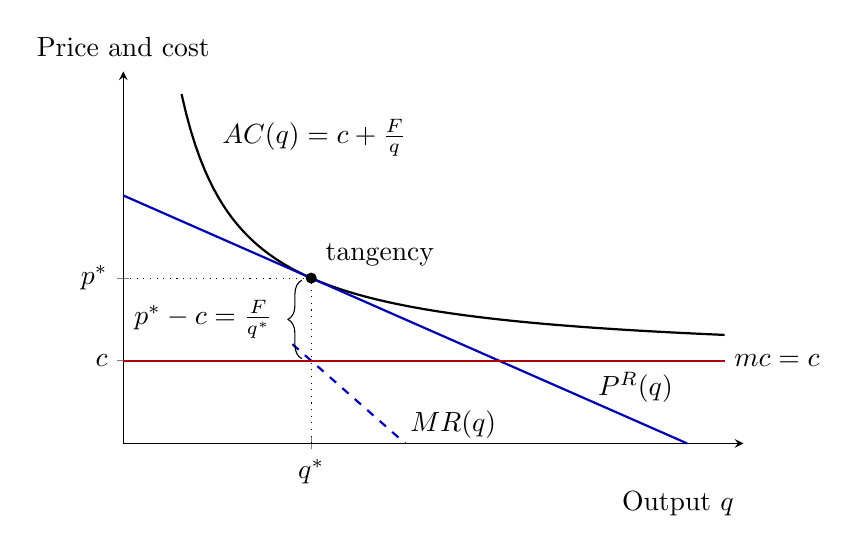
\begin{tikzpicture}
\begin{axis}[
  width=0.78\textwidth, height=0.52\textwidth,
  axis lines=left,
  xmin=0, xmax=6.6, ymin=0, ymax=9,
  xlabel={Output $q$}, ylabel={Price and cost},
  xtick={2}, xticklabels={$q^*$},
  ytick={2,4}, yticklabels={$c$,$p^*$},
  every axis x label/.style={at={(current axis.right of origin)}, anchor=north east, yshift=-14pt},
  every axis y label/.style={at={(current axis.above origin)}, anchor=south, yshift=2pt},
  clip=false]
  \addplot[thick, black, domain=0.62:6.4, samples=120] {2+4/x};
  \addplot[thick, blue!70!black, domain=0:6] {6-x};
  \addplot[thick, dashed, blue!70!black, domain=1.8:3] {6-2*x};
  \addplot[thick, red!70!black, domain=0:6.4] {2};
  \draw[dotted] (axis cs:2,0) -- (axis cs:2,4);
  \draw[dotted] (axis cs:0,4) -- (axis cs:2,4);
  \fill (axis cs:2,4) circle (2pt);
  \draw[decorate, decoration={brace, amplitude=5pt}] (axis cs:1.9,2.05) -- (axis cs:1.9,3.95)
    node[midway, left=7pt] {$p^* - c = \frac{F}{q^*}$};
  \node[anchor=west] at (axis cs:0.95,7.4) {$AC(q) = c + \frac{F}{q}$};
  \node[anchor=west] at (axis cs:4.95,1.35) {$P^R(q)$};
  \node[anchor=west] at (axis cs:2.95,0.45) {$MR(q)$};
  \node[anchor=west] at (axis cs:6.4,2) {$mc = c$};
  \node[anchor=south west] at (axis cs:2.05,4.05) {tangency};
\end{axis}
\end{tikzpicture}
\caption{The Chamberlin tangency under monopolistic competition. Free entry shifts the firm's inverse residual
demand $P^R(q)$ inward until it is tangent to average cost $AC(q) = c + \frac{F}{q}$ at $q^*$. There, marginal
revenue $MR(q)$ equals marginal cost $c$, and price equals average cost, so profit is zero. The markup
$p^* - c = \frac{F}{q^*}$ exactly covers the fixed cost. The curves are drawn for $c = 2$, $F = 4$ and
$P^R(q) = 6 - q$, which give $q^* = 2$ and $p^* = 4$.}
\label{fig:01-tangency}
\end{figure}

\citet[p.~1050]{Bresnahan1989} draws the welfare lesson. ``In the Chamberlinian tangency of monopolistic
competition, every firm has market power in the sense of this section. Yet that does not establish that there is
any inefficiency, once the need to cover the fixed costs of product design are taken into account.'' Forcing
every price down to marginal cost would leave each firm with a loss equal to its fixed cost, and some products
would disappear. Whether the market supplies too many or too few products depends on how much a product adds to
consumer surplus relative to the business it takes from rivals. Free entry can give too little variety under
monopolistic competition and too much entry in homogeneous-product markets \citep[see][and the work they
cite]{MankiwWhinston1986}. Bresnahan concludes that the welfare meaning of short-run market power with
differentiated products depends on the supply of new firms and new products. That supply is an empirical
question.

The same logic sits at the center of the recent debate over rising markups.
\citet{DeLoeckerEeckhoutUnger2020} estimate that the average ratio of price to marginal cost among US public
firms has risen since 1980. By \cref{prop:01-zero-profit-markup}, a higher markup need not mean higher profit if
fixed and overhead costs have risen as well. \Cref{sec:01-rising-markups} returns to this debate.

\subsection{The Cournot benchmark: concentration and margins}\label{sec:01-cournot-hhi}

We now have a measure of structure and a measure of market power. The simplest model that links them is the
Cournot model of quantity competition with a homogeneous good. Its central result motivates the cross-industry
regressions of \cref{sec:01-scp}. A small extension of the same result shows why those regressions are hard to
interpret.

\begin{assumption}[Homogeneous-good Cournot oligopoly]\label{ass:01-cournot}
\leavevmode
\begin{enumerate}[label=(\roman*)]
  \item There are $N$ firms selling a homogeneous good. Inverse market demand $P(Q)$ is twice differentiable,
  with $P'(Q) < 0$, where $Q = \sum_{i=1}^{N} q_i$.
  \item Firm $i$ has constant marginal cost $c_i$. It may also have a fixed cost, which does not affect its
  choice of output once it is active.
  \item Firms choose quantities simultaneously. Firm $i$ maximizes $\pi_i = \left(P(Q) - c_i\right) q_i$,
  taking its rivals' quantities as given.
  \item The equilibrium is interior. Every firm produces $q_i > 0$, and every firm's second-order condition
  $2P'(Q) + q_i P''(Q) < 0$ holds.
\end{enumerate}
\end{assumption}

\Cref{ch:theory} gives conditions for the existence and uniqueness of this equilibrium, and
\citet[Section~5.7.1]{Tirole1988} surveys them. Under mild boundary conditions, a pure-strategy equilibrium exists
when each firm's profit is concave in its own output, for which convex costs and concave demand suffice. With
two firms it is unique when the reaction functions have slopes below one in absolute value. Linear demand with
constant marginal cost gives the slope $-\frac{1}{2}$. Here we take an interior equilibrium as given. As in \cref{rem:01-residual}, the
market elasticity at the equilibrium is $\varepsilon = -\frac{P(Q)}{Q P'(Q)}$. Firm $i$'s Lerner index is
$L_i = \frac{P - c_i}{P}$, and the share-weighted average $\sum_i s_i L_i$ is the industry Lerner index.

\begin{proposition}[Cowling and Waterson]\label{prop:01-cowling-waterson}
Under \cref{ass:01-cournot}, every firm's Lerner index equals its market share divided by the market elasticity,
and the share-weighted Lerner index equals the Herfindahl-Hirschman index divided by the market elasticity:
\begin{equation}\label{eq:01-cowling-waterson}
  L_i = \frac{P - c_i}{P} = \frac{s_i}{\varepsilon}, \qquad \sum_{i=1}^{N} s_i L_i = \frac{\HHI}{\varepsilon} .
\end{equation}
\end{proposition}

\begin{proof}
Firm $i$'s first-order condition is
\[
  \frac{\partial \pi_i}{\partial q_i} = P(Q) + q_i P'(Q) - c_i = 0 .
\]
Rearrange it as $P - c_i = -q_i P'(Q)$ and divide by $P$:
\[
  \frac{P - c_i}{P} = -\frac{q_i P'(Q)}{P} .
\]
Multiply and divide the right side by $Q$:
\[
  \frac{P - c_i}{P} = \frac{q_i}{Q}\left(-\frac{Q P'(Q)}{P}\right) .
\]
The first factor is $s_i$ and the second is $\frac{1}{\varepsilon}$, which gives $L_i = \frac{s_i}{\varepsilon}$.
Multiply by $s_i$ and sum over firms:
\[
  \sum_{i=1}^{N} s_i L_i = \sum_{i=1}^{N} \frac{s_i^2}{\varepsilon} = \frac{\HHI}{\varepsilon} . \qedhere
\]
\end{proof}

The result is due to \citet{CowlingWaterson1976}. It fits together with the firm-level pricing rule. By
\eqref{eq:01-residual-elasticity}, firm $i$'s residual elasticity with rivals' output held fixed is
$\varepsilon^R_i = \frac{\varepsilon}{s_i}$, so
\[
  L_i = \frac{s_i}{\varepsilon} = \frac{1}{\varepsilon^R_i} .
\]
Each Cournot firm follows the inverse elasticity rule of \cref{prop:01-pricing-rule} for its own residual demand.
Large firms face less elastic residual demand and set higher margins. Since a firm's output and its margin are
chosen together, low-cost firms are both large and high-margin. \Cref{sec:01-demsetz} develops this observation
into the efficiency critique of regressions of profitability on concentration.

The same result links concentration to industry profit \citep[Section~5.5, eq.~5.14 and Exercise~5.6]{Tirole1988}.
Industry variable profit is
\[
  \Pi = \sum_{i=1}^{N} (P - c_i)\, q_i = \sum_{i=1}^{N} P L_i\, s_i Q = PQ \sum_{i=1}^{N} s_i L_i
  = \frac{PQ}{\varepsilon}\,\HHI .
\]
The second equality uses $P - c_i = P L_i$ and $q_i = s_i Q$, and the last uses \eqref{eq:01-cowling-waterson}.
The ratio of industry variable profit to industry revenue is therefore $\frac{\HHI}{\varepsilon}$. Suppose further
that demand has unit elasticity, $Q = \frac{k}{P}$ for a constant $k > 0$, so that consumers spend the fixed
amount $k$ on the good. Then $PQ = k$ and $\Pi = k\,\HHI$, which is Tirole's equation (5.15). In this case the
index measures industry profitability exactly, up to the constant $k$.

\begin{corollary}[Special cases]\label{cor:01-cournot-cases}
Under \cref{ass:01-cournot}, the following hold.
\begin{enumerate}[label=(\roman*)]
  \item With symmetric costs $c_i = c$, every firm has share $\frac{1}{N}$, $\HHI = \frac{1}{N}$, and
  $L = \frac{P - c}{P} = \frac{1}{N\varepsilon}$.
  \item With $N = 1$, $L = \frac{1}{\varepsilon}$, the monopoly inverse elasticity rule.
  \item With symmetric costs and an equilibrium elasticity bounded away from zero, $L \to 0$ and $P \to c$ as
  $N \to \infty$.
\end{enumerate}
\end{corollary}

\begin{proof}
With equal costs, the first-order conditions $P - c = -q_i P'(Q)$ have the same left side for every firm, so all
firms produce the same output and $s_i = \frac{1}{N}$. Then $\HHI = N \cdot \frac{1}{N^2} = \frac{1}{N}$, and all
the $L_i$ are equal to $L$, so \eqref{eq:01-cowling-waterson} gives (i). Setting $N = 1$ in (i) gives (ii). For
(iii), $L = \frac{1}{N\varepsilon}$ goes to zero when $\varepsilon$ stays above a positive constant, and
$L = 1 - \frac{c}{P} \to 0$ means $P \to c$.
\end{proof}

Statement (iii) is the sense in which Cournot competition approaches perfect competition as the number of firms
grows. The Cournot model therefore generates the hypothesis behind a generation of empirical work, namely that
margins rise with concentration. Read literally, \eqref{eq:01-cowling-waterson} suggests regressing the average
margin of each industry on its $\HHI$ across industries, with slope $\frac{1}{\varepsilon}$.

The Cournot result fixes the form of competition. To see what happens when conduct varies, we use a device from
the older literature. Suppose firm $i$ chooses its output as if its rivals' total output $Q_{-i} = Q - q_i$
responded to its own output at the rate
\[
  r_i = \frac{\dd Q_{-i}}{\dd q_i} .
\]
The number $r_i$ is firm $i$'s \emph{conjectural variation}. The firm then perceives
$\frac{\dd Q}{\dd q_i} = 1 + r_i$. Cournot behavior is $r_i = 0$.

\begin{proposition}[Margins and concentration under general conduct]\label{prop:01-clarke-davies}
Keep \cref{ass:01-cournot}, except that firm $i$ maximizes profit under the conjectural variation $r_i$, with
$1 + r_i \ge 0$. Then
\begin{equation}\label{eq:01-cv-lerner}
  L_i = \frac{s_i (1 + r_i)}{\varepsilon}, \qquad
  \sum_{i=1}^{N} s_i L_i = \frac{\theta}{\varepsilon}, \qquad
  \theta = \sum_{i=1}^{N} s_i^2 (1 + r_i) .
\end{equation}
Suppose conjectures are proportional, as in \citet{ClarkeDavies1982}. Firm $i$ expects every rival $j \ne i$ to
change its output by $\kappa$ times firm $i$'s own percentage change, for some $\kappa \in [0, 1]$. Then
\begin{equation}\label{eq:01-clarke-davies}
  r_i = \kappa\,\frac{1 - s_i}{s_i}, \qquad
  L_i = \frac{\kappa + (1 - \kappa)s_i}{\varepsilon}, \qquad
  \sum_{i=1}^{N} s_i L_i = \frac{\kappa + (1 - \kappa)\HHI}{\varepsilon} .
\end{equation}
\end{proposition}

\begin{proof}
Under the conjecture, firm $i$ perceives $\frac{\dd Q}{\dd q_i} = 1 + r_i$, so its perceived marginal profit is
\[
  \frac{\dd \pi_i}{\dd q_i} = P(Q) + q_i P'(Q) \frac{\dd Q}{\dd q_i} - c_i = P(Q) + q_i P'(Q)(1 + r_i) - c_i .
\]
Setting it to zero and following the steps in the proof of \cref{prop:01-cowling-waterson},
\begin{align}
  P + P'(Q)\, q_i (1 + r_i) &= c_i, \label{eq:01-cv-foc}\\
  \frac{P - c_i}{P} &= \frac{q_i}{Q}\left(-\frac{Q P'(Q)}{P}\right)(1 + r_i), \notag\\
  L_i &= \frac{s_i (1 + r_i)}{\varepsilon} . \notag
\end{align}
Multiplying by $s_i$ and summing gives
$\sum_i s_i L_i = \frac{1}{\varepsilon}\sum_i s_i^2 (1 + r_i) = \frac{\theta}{\varepsilon}$.

In the proportional case, the conjecture is $\frac{\dd q_j}{q_j} = \kappa\,\frac{\dd q_i}{q_i}$ for every
$j \ne i$, that is, $\frac{\dd q_j}{\dd q_i} = \kappa\,\frac{q_j}{q_i}$. Summing over rivals,
\[
  r_i = \sum_{j \ne i} \frac{\dd q_j}{\dd q_i} = \kappa\,\frac{Q_{-i}}{q_i} = \kappa\,\frac{Q - q_i}{q_i}
  = \kappa\,\frac{1 - s_i}{s_i} .
\]
Then
\[
  s_i (1 + r_i) = s_i + \kappa (1 - s_i) = \kappa + (1 - \kappa) s_i ,
\]
which gives the firm-level formula. Multiplying by $s_i$ and summing over firms,
\begin{align*}
  \theta = \sum_{i=1}^{N} s_i^2 (1 + r_i) &= \sum_{i=1}^{N} \left(\kappa s_i + (1 - \kappa) s_i^2\right) \\
  &= \kappa \sum_{i=1}^{N} s_i + (1 - \kappa) \sum_{i=1}^{N} s_i^2 \\
  &= \kappa + (1 - \kappa)\HHI ,
\end{align*}
where the last line uses $\sum_i s_i = 1$.
\end{proof}

The parameter $\theta$ is the index of industry conduct that we use throughout the book. Price-taking behavior,
$r_i = -1$ for every firm, gives $\theta = 0$ and $L_i = 0$. Cournot behavior, $r_i = 0$, gives
$\theta = \HHI$, which equals $\frac{1}{N}$ when firms are symmetric. In the Clarke-Davies family, $\kappa = 0$
is Cournot behavior and $\kappa = 1$ is joint profit maximization. With $\kappa = 1$ the firm expects all rivals
to move in proportion, so $1 + r_i = \frac{1}{s_i}$ and $q_i(1 + r_i) = Q$. Condition \eqref{eq:01-cv-foc} then
becomes $P + Q P'(Q) = c_i$, the first-order condition of a monopolist. With constant marginal costs, these
conditions can hold for all active firms only if their costs are equal, and the split of output among them is then
indeterminate. Every firm has $L_i = \frac{1}{\varepsilon}$ and $\theta = 1$. With rising marginal costs, as in
\cref{prop:01-supply-relation}, the same conditions equalize marginal costs across firms, as joint profit
maximization requires. Summing \eqref{eq:01-cv-foc} with weights $s_i$ gives the industry relation
\begin{equation}\label{eq:01-industry-relation}
  P = \bar c - \theta\, Q P'(Q), \qquad \bar c = \sum_{i=1}^{N} s_i c_i ,
\end{equation}
because $\sum_i s_i q_i (1 + r_i) = Q\sum_i s_i^2(1 + r_i) = Q\theta$. \Cref{sec:01-conduct-parameter} calls
\eqref{eq:01-industry-relation} the supply relation and shows how the New Empirical Industrial Organization is
built around it.

Conjectural variations must be read with care. In a static game a firm moves once and never observes a response,
so a ``conjecture'' about its rivals' reactions has no behavioral content within the game. The parameter
$\theta$ is best read as an index of how close the outcome is to the collusive one. \citet{Bresnahan1989}
stresses this reading, and \cref{sec:01-conduct-parameter} explains it. \Cref{ch:theory} discusses the theory of
conjectural variations and the conduct parameter.

\Cref{prop:01-clarke-davies} contains the main message of this section. In the Clarke-Davies family the average
margin is a linear function of the index,
\begin{equation}\label{eq:01-cd-line}
  \sum_{i=1}^{N} s_i L_i = \frac{\kappa}{\varepsilon} + \frac{1 - \kappa}{\varepsilon}\,\HHI ,
\end{equation}
with intercept $\frac{\kappa}{\varepsilon}$ and slope $\frac{1 - \kappa}{\varepsilon}$. Both depend on conduct and
on the demand elasticity. The slope is largest under Cournot behavior. It is zero under collusion, where margins
are at the monopoly level whatever the concentration. Panel (a) of \cref{fig:01-lerner-hhi} plots
\eqref{eq:01-cd-line} for $\varepsilon = 2$. The slope of margins on concentration is therefore no constant of
nature shared by all industries. This is at once the theoretical case for regressing margins on concentration
and the first reason such regressions fail. Industries differ in their elasticities and their conduct, and these
differences are correlated with concentration in ways that \cref{sec:01-scp-econometrics} explores.

Even within one industry with fixed conduct, the relation need not be linear, because the elasticity changes
with concentration. Take linear inverse demand $P(Q) = a - bQ$ with $a > c > 0$ and $b > 0$, and $N$ symmetric
Cournot firms with marginal cost $c$. The first-order condition $a - bQ - bq_i - c = 0$ holds for every firm, so
outputs are equal and $q_i = \frac{Q}{N}$. Summing the conditions over firms and solving,
\begin{align*}
  N(a - c) - NbQ - bQ &= 0, \\
  Q &= \frac{N(a - c)}{b(N + 1)}, \\
  P = a - bQ &= \frac{a + Nc}{N + 1} .
\end{align*}
The Lerner index and the market elasticity at the equilibrium are
\begin{align*}
  L &= \frac{P - c}{P} = \frac{\frac{a - c}{N + 1}}{\frac{a + Nc}{N + 1}} = \frac{a - c}{a + Nc}, \\
  \varepsilon &= \frac{P}{bQ} = \frac{a + Nc}{N(a - c)} .
\end{align*}
Substitute $N = \frac{1}{\HHI}$ and multiply each numerator and denominator by $\HHI$:
\begin{equation}\label{eq:01-linear-cournot-LH}
  L = \frac{(a - c)\HHI}{a\HHI + c}, \qquad \varepsilon = \frac{a\HHI + c}{a - c} .
\end{equation}
As a check, $\frac{\HHI}{\varepsilon} = \frac{(a - c)\HHI}{a\HHI + c} = L$, as \cref{prop:01-cowling-waterson}
requires. The elasticity rises with concentration, because fewer firms means a higher price and a lower quantity
along a linear demand curve. Differentiating $L$ with respect to $\HHI$,
\begin{align*}
  \frac{\dd L}{\dd \HHI} &= \frac{(a - c)(a\HHI + c) - (a - c)\HHI \cdot a}{(a\HHI + c)^2}
  = \frac{c(a - c)}{(a\HHI + c)^2} > 0, \\
  \frac{\dd^2 L}{\dd \HHI^2} &= -\frac{2ac(a - c)}{(a\HHI + c)^3} < 0 .
\end{align*}
The margin rises with concentration at a decreasing rate. Panel (b) of \cref{fig:01-lerner-hhi} plots the curve
for two values of the ratio $\frac{c}{a}$. A higher ratio of marginal cost to the demand intercept lowers the
whole curve. Industries with different cost-demand ratios lie on different curves, so even the causal effect of
concentration on margins differs across industries. Throughout this calculation $N$ is fixed. When entry
determines $N$, concentration becomes an equilibrium outcome itself, a problem that \cref{sec:01-endogeneity}
takes up.

\begin{figure}[htbp]
\centering
\begin{subfigure}[t]{0.49\textwidth}
\centering
\begin{tikzpicture}[baseline=(current axis.north)]
\begin{axis}[
  scale only axis, width=0.78\linewidth, height=0.66\linewidth,
  xmin=0, xmax=1, ymin=0, ymax=0.6,
  xlabel={$\HHI$}, ylabel={$\sum_i s_i L_i$},
  xtick={0,0.25,0.5,0.75,1}, ytick={0,0.1,0.2,0.3,0.4,0.5,0.6},
  tick label style={font=\footnotesize}, label style={font=\small},
  domain=0:1, samples=2,
  legend columns=2,
  legend style={font=\footnotesize, at={(0.5,-0.24)}, anchor=north, draw=none, column sep=4pt},
  legend cell align=left]
  \addplot[thick, black] {x/2};
  \addlegendentry{$\kappa = 0$ (Cournot)}
  \addplot[thick, blue!70!black, dashed] {(0.25+0.75*x)/2};
  \addlegendentry{$\kappa = 0.25$}
  \addplot[thick, red!70!black, densely dotted] {(0.5+0.5*x)/2};
  \addlegendentry{$\kappa = 0.5$}
  \addplot[thick, green!45!black, dashdotted] {0.5};
  \addlegendentry{$\kappa = 1$ (collusion)}
\end{axis}
\end{tikzpicture}
\caption{Clarke-Davies conduct, $\varepsilon = 2$}
\end{subfigure}\hfill
\begin{subfigure}[t]{0.49\textwidth}
\centering
\begin{tikzpicture}[baseline=(current axis.north)]
\begin{axis}[
  scale only axis, width=0.78\linewidth, height=0.66\linewidth,
  xmin=0, xmax=1, ymin=0, ymax=0.75,
  xlabel={$\HHI$}, ylabel={$L$},
  xtick={0,0.25,0.5,0.75,1}, ytick={0,0.1,0.2,0.3,0.4,0.5,0.6,0.7},
  tick label style={font=\footnotesize}, label style={font=\small},
  domain=0:1, samples=101,
  legend columns=2,
  legend style={font=\footnotesize, at={(0.5,-0.24)}, anchor=north, draw=none, column sep=4pt},
  legend cell align=left]
  \addplot[thick, black] {8*x/(10*x+2)};
  \addlegendentry{$\frac{c}{a} = 0.2$}
  \addplot[thick, blue!70!black, dashed] {5*x/(10*x+5)};
  \addlegendentry{$\frac{c}{a} = 0.5$}
  \addplot[only marks, mark=*, mark size=1.3pt, black,
    samples at={1,0.5,0.333333,0.25,0.2,0.166667,0.142857,0.125,0.111111,0.1}]
    {8*x/(10*x+2)};
  \addlegendentry{$\HHI = \frac{1}{N}$}
  \addplot[only marks, mark=*, mark size=1.3pt, blue!70!black,
    samples at={1,0.5,0.333333,0.25,0.2,0.166667,0.142857,0.125,0.111111,0.1}, forget plot]
    {5*x/(10*x+5)};
\end{axis}
\end{tikzpicture}
\caption{Symmetric Cournot, linear demand}
\end{subfigure}
\caption{Margins and concentration. Panel (a) plots the share-weighted Lerner index against the
Herfindahl-Hirschman index in the Clarke-Davies family,
$\sum_i s_i L_i = \frac{\kappa + (1 - \kappa)\HHI}{\varepsilon}$, for $\varepsilon = 2$. The lines run from
$\left(0, \frac{\kappa}{\varepsilon}\right)$ to $\left(1, \frac{1}{\varepsilon}\right)$. Panel (b) plots the
symmetric Cournot relation with linear demand, $L = \frac{(a - c)\HHI}{a\HHI + c}$, for $\frac{c}{a} = 0.2$ and
$\frac{c}{a} = 0.5$. Dots mark $\HHI = \frac{1}{N}$ for $N = 1, \dots, 10$.}
\label{fig:01-lerner-hhi}
\end{figure}
